\documentclass[10pt,a4paper]{article}
\usepackage[margin=0.7in]{geometry}
\usepackage[utf8]{inputenc}
\usepackage[T1]{fontenc}
\usepackage{lmodern,microtype,booktabs,graphicx,amsmath,hyperref,enumitem,caption}
\captionsetup{font=small,labelfont=bf,skip=3pt}
\setlist{nosep,leftmargin=1.2em}
\hypersetup{colorlinks=true,urlcolor=blue,linkcolor=black,citecolor=black}
\setlength{\parskip}{3pt}\setlength{\parindent}{0pt}
\title{\vspace{-1.2em}\large\textbf{When should a constrained-selection grounding pipeline escalate to a human?\\ A post-hoc risk--coverage study on topic-to-timestamp alignment}\vspace{-0.6em}}
\author{Abdul Mannan}\date{22 November 2026}
\begin{document}\maketitle\vspace{-1.4em}
\begin{abstract}\small\noindent
Yılbırt, Litvak and Färber \cite{yilbirt} replace free-form timestamp generation by \emph{selecting} one retrieved transcript candidate, which reduces invalid outputs, yet GPT-5.4 is within 30\,s of the annotated start for only 34.3\,\% of 420 queries. I ask what happens if the system may \emph{abstain and escalate to a human}. Using only the per-query outputs released with their artifact (no transcripts), I compare abstention rules and a small PyTorch deferral head in a risk--coverage framework \cite{chow,geifman}. Agreement between two selectors raises accuracy among accepted answers from 34.3\,\% to 41.5\,\% at 50.5\,\% coverage, but 43\,\% of those answers are still more than 5\,min off. The predicted position in the meeting is about as informative as agreement. A logistic head on nine inference-time features closes about two thirds of the AURC gap between random and oracle abstention and is the only policy clearly better than a simple vote rule. The analysis is post hoc, on the same 420 queries, and should be read as a pilot.
\end{abstract}

\section{Question and setting}
A pipeline that must return a timestamp can fail silently: the selected candidate is plausible but several minutes from the annotated boundary. If wrong answers cannot be avoided, the practical question is which answers to hand to a human. This is the selective-prediction setting: accept an answer when a confidence score is high, and measure \emph{risk} (error rate among accepted answers) against \emph{coverage} (share accepted) \cite{chow,geifman}. It mirrors, as an analogy only, designs in which rule-based decisions fall back to memory and finally to a human when no reliable decision is possible.

\textbf{Data.} The upstream artifact \cite{repo} (commit \texttt{63ffb7a}) releases an annotation layer plus sanitized per-query results: gold timestamp, predicted timestamp and selected candidate ID for 420 queries on 196 recordings, for four systems: Mistral-7B and GPT-5.4 with Chunk-ID selection (hybrid BM25/dense retrieval, 90\,s/45\,s windows) and with free-form timestamp generation (dense retrieval, 30\,s/15\,s windows). It contains no transcripts, retrieval scores or model confidences, so the original pipeline was \emph{not} re-run and no new model outputs exist. An answer is \emph{correct} if within 30\,s of gold (the paper's Exact@30s). My re-derived Exact@30s, MAE, median error and parsed counts match the paper for all four systems (e.g.\ GPT-5.4 Chunk-ID: 0.343, 743.4\,s; Mistral-7B: 0.300, 761.0\,s).

\section{Method}
The served answer is the GPT-5.4 Chunk-ID prediction (Mistral-7B as a robustness check). Unparsed outputs are always escalated. Policies:
\begin{itemize}
\item \textbf{Random} abstention (chance reference) and an \textbf{oracle} that accepts all correct answers first (upper bound).
\item \textbf{Rules:} (i) disagreement $|t_{\text{Mistral}}-t_{\text{GPT-5.4}}|$ between the two Chunk-ID selectors; (ii) \emph{votes}: number (0--3) of the other three systems within 30\,s of the served answer; (iii) earlier candidate index.
\item \textbf{Learned deferral head (PyTorch):} logistic regression or one hidden layer of 16 ReLU units predicting P(correct) from nine inference-time features (log-differences to the other systems' predictions, their parse flags, votes, selected candidate index, log predicted time). Binary cross-entropy with class weight, Adam (lr 0.02, weight decay $10^{-3}$, 300 full-batch epochs). Evaluation is \emph{out-of-fold}: 5 folds grouped by recording, 10 repeats. Gold timestamps are used only to form labels.
\end{itemize}
Metrics: risk--coverage curves (random tie-breaking), area under the curve (AURC, lower is better), Exact@30s among accepted answers, share of accepted answers with error $>$5\,min, and the shares of wrong answers reaching a human and of right answers escalated needlessly. Paired bootstrap over queries (500 resamples for AURC differences, 1000 for threshold intervals). A label-permutation check gives AUC 0.50 against the permuted labels.

\section{Results}
\begin{table}[h]\centering\small
\begin{tabular}{lcccc}\toprule
Policy (served: GPT-5.4 Chunk-ID, $n{=}420$) & AURC $\downarrow$ & @50\,\% & @70\,\% & @90\,\% \\\midrule
Random abstention & 0.656 & 0.343 & 0.357 & 0.349\\
Rule: Mistral/GPT-5.4 agreement & 0.599 & 0.415 & 0.401 & 0.362\\
Rule: votes (others within 30\,s) & 0.505 & 0.500 & 0.426 & 0.372\\
Head, agreement features only & 0.493 & 0.529 & 0.449 & 0.373\\
Head, predicted position only & 0.464 & 0.490 & 0.446 & 0.378\\
Head, logistic, all 9 features & \textbf{0.413} & \textbf{0.571} & 0.459 & 0.376\\
Head, MLP, all 9 features & 0.433 & 0.533 & 0.449 & 0.370\\
Oracle (upper bound) & 0.291 & 0.686 & 0.490 & 0.381\\\bottomrule
\end{tabular}
\caption{AURC and Exact@30s among accepted answers at 50/70/90\,\% coverage. Without abstention Exact@30s is 0.343.}\label{tab}\end{table}

\begin{figure}[h]\centering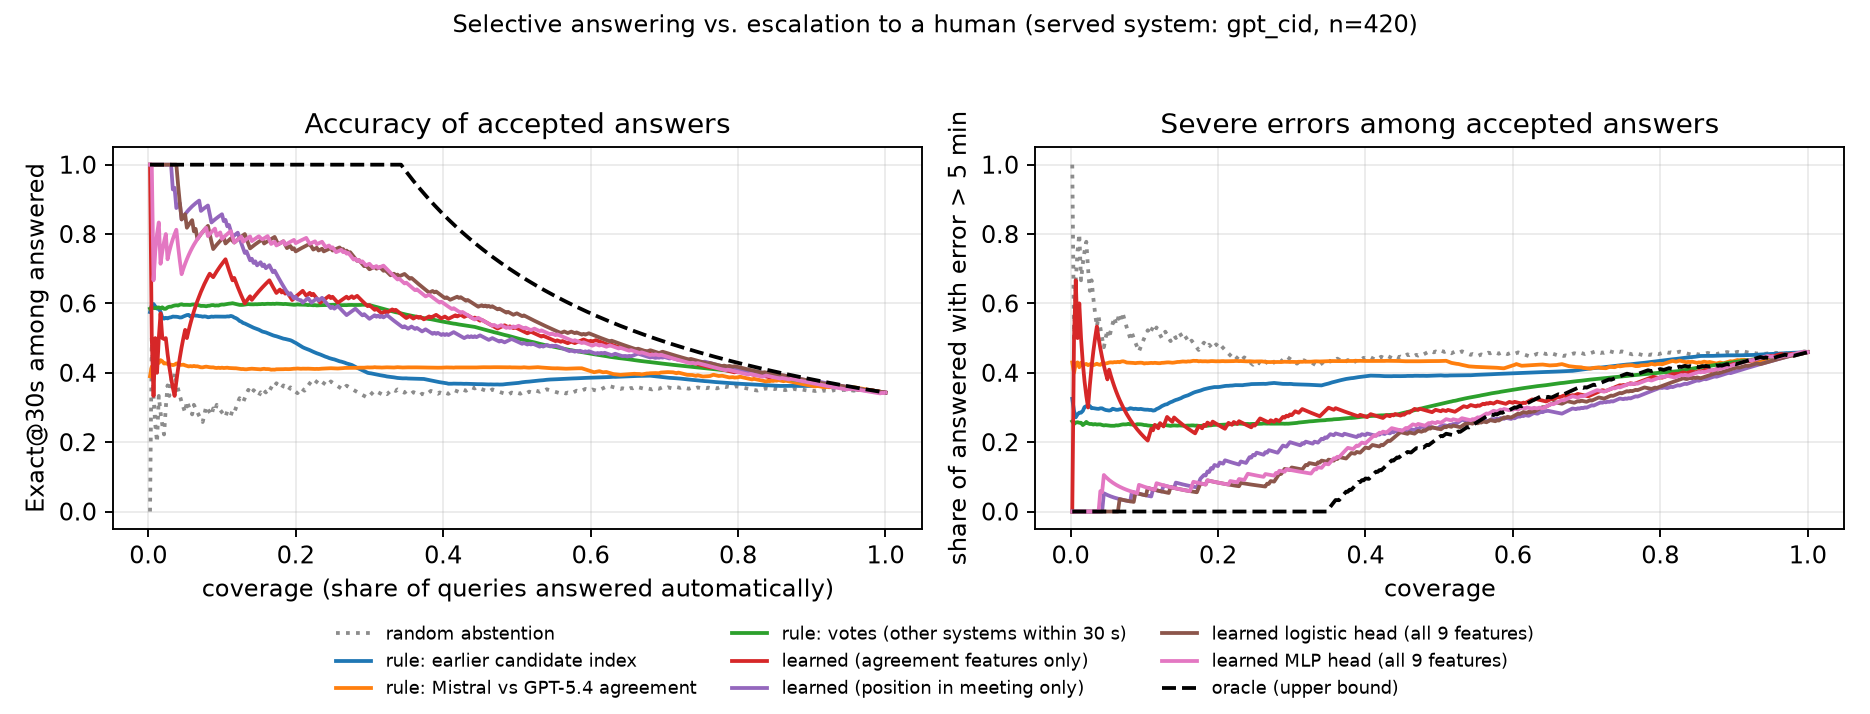
\includegraphics[width=0.8\linewidth]{risk_coverage.png}
\caption{Risk--coverage for the policies in Table~\ref{tab}: accuracy (left) and share of severe errors ($>$5\,min, right) among accepted answers.}\end{figure}

\textbf{Agreement helps modestly.} Accepting only exact agreement of the two selectors (coverage 0.505) gives Exact@30s 0.415 (95\,\% CI 0.344--0.484), sends 55\,\% of wrong answers to a human, and escalates 39\,\% of right ones. Yet 43\,\% of the accepted answers are more than 5\,min off: both selectors often choose the same wrong candidate. Loosening the tolerance to 30\,s gives coverage 0.726 and Exact@30s 0.397.

\textbf{Position matters as much.} Answers predicted in the first 88\,s are correct 60\,\% of the time, those after about 21\,min only 6.7\,\% (single-feature AUC 0.75 for the predicted time; 0.73 for votes).

\textbf{Combining signals.} The logistic head (AURC 0.413) closes about two thirds of the gap between random (0.656) and oracle (0.291). Against the votes rule, only this head is clearly better (paired $\Delta$AURC $-0.092$, 95\,\% CI $-0.123$ to $-0.059$); the agreement-only ($-0.012$ [$-0.040$, $+0.016$]) and position-only ($-0.042$ [$-0.088$, $+0.008$]) heads are not distinguishable from it. The MLP is not better than logistic regression. With Mistral-7B as served system the all-feature head is again best (AURC 0.464; random 0.707, oracle 0.339), but the order of the single-signal policies changes.

\section{Limitations and relation to verifiable pipelines}
\begin{itemize}
\item \textbf{Post hoc, one benchmark.} Feature groups, ablations and the votes comparison were chosen after seeing earlier runs (\texttt{RUNLOG.md}); folds are grouped by recording but no untouched test set exists. Gold labels come from a single annotator (upstream limitation); municipal meetings only.
\item \textbf{No confidence signals.} Logits, retrieval scores and transcript text were not released, so likely stronger signals are unused. The position feature reflects this benchmark and may not transfer.
\item \textbf{Cost.} Agreement requires at least two neural calls per query; this study measures escalation quality, not savings in model calls.
\item \textbf{Next steps.} Re-run the pipeline on reconstructed transcripts to log selector probabilities and retrieval margins, evaluate on held-out recordings, and test rule-first routing in which a cheap check decides when a model is called at all.
\end{itemize}
\textbf{Reproducibility.} \texttt{bash run.sh} (CPU only, about 5 min) re-creates every number and the figure from the pinned upstream commit; the repository holds the code, tests and a plain run log including failures.

\footnotesize\begin{thebibliography}{9}
\bibitem{yilbirt} Z.\ Yılbırt, M.\ Litvak, M.\ Färber. \emph{Topic-to-Timestamp Alignment by Constrained Evidence Selection.} arXiv:2606.20890, 2026.
\bibitem{repo} Code \& data of \cite{yilbirt}: \url{https://github.com/faerber-lab/topic-timestamp-alignment} (code MIT; annotations CC BY 4.0).
\bibitem{chow} C.\ K.\ Chow. On optimum recognition error and reject tradeoff. \emph{IEEE Trans.\ Information Theory} 16(1):41--46, 1970.
\bibitem{geifman} Y.\ Geifman, R.\ El-Yaniv. Selective classification for deep neural networks. \emph{NeurIPS}, 2017.
\end{thebibliography}
\end{document}
